\chapter{一些实例}
\label{chap:example}
\section{插入图片}
\begin{figure}[htbp]
  \centering
  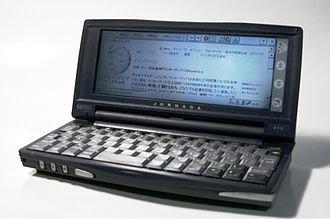
\includegraphics[width=0.8\textwidth]{images/examples/330px-Jornada_690_HP_d.jpg} \\
  \caption[早期的智能手机]{HP Jornada 690开启了手机和电脑结合的早期概念,成为智能手机早期概念范例。} 
  \label{fig:lengthscale}
\end{figure}


\section{引用}
不同的论文引用方式。
也可以引用公示(\cref{eq:log}),引用表格(见\cref{tab:schedule}),引用图片(见\cref{fig:lengthscale}),等等。

对于论文的引用:单个引用\cite{erdHos1960evolution},多个引用\cite{erdHos1960evolution,konect:socialcomputing,konect}。

\section{插入表格}
引用表格(见\cref{tab:schedule})。
\begin{table}[htbp]
	\caption{计划进度}  
	\label{tab:schedule}
	\centering
	\scalebox{0.9}{
		\begin{tabular}{lll}
		  \toprule
		  \multicolumn{3}{c}{进度}\\
		  \midrule
		   2007.10~--~2008.05 & & 完成文献综述和开题报告\\
		  
		  2008.05~--~2008.07 & & 完成电渗流多尺度模拟的理论构建和初步模型验证,\\
		                   & & 同时开始写毕业论文\\
		  2008.07~--~2008.10 & & 完成模型验证,并进行多种条件下电渗流(泵)的仿真模拟,\\
		                    & & 实验数据处理,制表,论文书写\\
		  2008.10~--~2008.12 & & 完成所有仿真对象的模拟,并计划完成毕业论文的初稿\\
		  2008.12~--~2009.03 & & 完成论文修改\\
		  2009.03~--~2009.05  & & 准备答辩、答辩\\
		  \bottomrule
		\end{tabular}
	}
\end{table}

\section{插入公式}
\begin{dotsequation}
    \begin{aligned}
		                     a&=b\\
		                     c&=d\\
		                  2x+y&=6\\
		                     x&=4y+\log (y)\\
		\sum_i^{10} i \times x&=y
    \end{aligned}
    \label{eq:log}
\end{dotsequation}


\section{插入算法}
尝试插入算法(见\autoref{alg:alg1})

\begin{algorithm}[htbp]
    \setstretch{1.3}
    \textbf{Input:} 两个数 $n$, $k$
    \begin{algorithmic}[1]
        \STATE 初始化 $s$ 为 $0$ \label{algline:init}
        \FOR{$i = 1,2,...,k$}    \COMMENT{\textbf{循环}}
        \label{algline:for} 
        \IF {$i\;\% \;5\neq 0$}
        \STATE $s=s+n+i$
        \ENDIF 
        \ENDFOR \label{algline:endfor}
        \STATE \textbf{return} $s$ \label{algline:return} 
    \end{algorithmic}
    \caption{sum($n$, $k$)}
    \label{alg:alg1}
\end{algorithm}

\section{插入代码}
\definecolor{commentColor}{rgb}{0.0, 0.5, 0.0}
\lstset{ %
    language=Python,                % the language of the code
    basicstyle=\scriptsize\ttfamily,           % the size of the fonts that are used for the code
    numbers=left,                   % where to put the line-numbers
    numberstyle=\tiny\color{gray},  % the style that is used for the line-numbers
    stepnumber=2,                   % the step between two line-numbers. If it's 1, each line 
    % will be numbered
    numbersep=5pt,                  % how far the line-numbers are from the code
    backgroundcolor=\color{white},      % choose the background color. You must add \usepackage{color}
    showspaces=false,               % show spaces adding particular underscores
    showstringspaces=false,         % underline spaces within strings
    showtabs=false,                 % show tabs within strings adding particular underscores
    rulecolor=\color{black},        % if not set, the frame-color may be changed on line-breaks within not-black text (e.g. commens (green here))
    tabsize=2,                      % sets default tabsize to 2 spaces
    captionpos=b,                   % sets the caption-position to bottom
    breaklines=true,                % sets automatic line breaking
    breakatwhitespace=false,        % sets if automatic breaks should only happen at whitespace
                 % show the filename of files included with \lstinputlisting;
    % also try caption instead of title
    keywordstyle=\color{blue},          % keyword style
    commentstyle=\color{commentColor},       % comment style
    stringstyle=\color{mauve},         % string literal style
    escapeinside={(*}{*)},            % if you want to add LaTeX within your code
    morekeywords={*,...}               % if you want to add more keywords to the set
}
\newcommand{\commentMath}[1]{$\color{commentColor}#1$}
\begin{lstlisting}
def func(n, k):
    """
    param n: 起始值 (*\commentMath{n}*)
    param k: 计数 (*\commentMath{k}*)
    """
    s=0
    for i in range(1,k):
        if i % 5 != 0:
            s = s+n+i
    return s
\end{lstlisting}
